\documentclass{article}
\usepackage[submission]{neurips_2026}
\usepackage[utf8]{inputenc}
\usepackage[T1]{fontenc}
\usepackage{graphicx}
\usepackage{booktabs}
\usepackage{amssymb}
\usepackage{amsmath}
\usepackage{hyperref}
\usepackage{caption}
\usepackage{tikz}
\usetikzlibrary{positioning,arrows.meta}

\title{When More Reward Signal Does Not Help: A Controlled Study of Reward Decomposition for GRPO Debugging}
\author{Anonymous Authors}

\begin{document}

\maketitle

\begin{center}
\textit{Code, dataset, per-bug results, and pre-registration: see anonymized supplementary material.}
\end{center}

\vspace{0.3cm}
\noindent \textbf{Keywords:} reinforcement learning, reward shaping, GRPO, program repair, verifiable rewards, generalization, negative results, evaluation methodology
\vspace{0.3cm}

\begin{abstract}
Hand-crafted reward decompositions are often used in reinforcement learning for language models to provide intermediate learning signals before a policy reliably achieves verifiable outcomes. We test whether such reasoning-targeted shaping improves GRPO training for program debugging. We train Qwen2.5-Coder-3B-Instruct with GRPO and LoRA on 90 single-function Python bugs under three reward configurations: a seven-component dense reward (R0), a graded executable outcome reward with regression penalties (R1), and a dense reward with the two reasoning-targeted components removed (R2). All three RL configurations share the same model, data, prompts, optimizer, curriculum, and evaluation procedure. On 90 held-out bugs, R0 achieves a 45.6\% solve rate, compared with 48.5\% for R1 and 48.5\% for R2. Paired bootstrap analysis gives a 95\% interval of [$-$8.5, $+$2.6] percentage points for R0$-$R1, providing no evidence that the dense reward improves final debugging success. The nine RL runs have a pooled mean held-out solve rate 9.7 percentage points [1.0, 18.5] above the zero-shot structured baseline (37.8\%). Despite producing substantially fewer degenerate GRPO groups, the dense reward does not translate its additional reward signal into a higher held-out solve rate. An external evaluation on 27 adapted QuixBugs programs yields solve rates between 39.5\% and 44.4\%, showing that the policies do not collapse on out-of-distribution code; however, without an external zero-shot baseline, these measurements remain descriptive and do not demonstrate an RL-induced generalization gain. The results provide no evidence, in this setting, that elaborate reasoning-targeted reward engineering is necessary when executable outcome supervision is already available.
\end{abstract}

\section{Introduction}
Reinforcement learning from verifiable rewards has become an increasingly common approach to improving language-model performance on tasks with checkable outcomes, including mathematics and code \cite{Shao2024, Guo2025}. A recurring design question in these systems is how much reward decomposition is useful beyond executable outcomes. Although test execution provides a verifiable signal, sampled fixes can produce similar test outcomes within a GRPO group, leaving little relative reward variation. A natural response is to decompose the reward into hand-crafted components that pay for intermediate desiderata: emitting the required format, stating a specific hypothesis about the fault, naming the buggy function, or resembling the reference solution. The implicit claim is that these additional signals provide useful within-group resolution before the policy reliably produces passing fixes.

The question is not whether dense rewards can increase the numerical reward assigned to intermediate behavior. They obviously can. The question is whether these additional signals improve the policy's eventual ability to produce test-passing fixes when the executable outcome remains available. We therefore hold the model, prompts, data, optimizer, curriculum, and evaluation fixed and vary only the reward decomposition. Because our setting is single-turn (the model produces the entire proposed fix in one completion), intermediate reasoning is not itself an environment transition. The dense components therefore shape the scalar reward assigned to a complete response rather than providing feedback at intermediate debugging steps.

We test this claim directly in a setting small enough to control completely. We built a debugging environment in which every candidate fix executes in a hardened sandbox against the bug's test cases, and a seven-component dense reward (R0) is implemented as a set of component ceilings on a single scoring class. An ablation is therefore a configuration, not a fork: R1 zeroes every shaping component and rescales the test-outcome term to the same range; R2 zeroes exactly the two reasoning-targeted components and keeps the rest. The three configurations were pre-registered, together with the hypotheses, statistical tests, and threats to validity, before any experiment ran.

On 90 held-out bugs, we find no statistically detectable difference between the reward configurations. The graded outcome reward matches or slightly exceeds the full dense reward, and no pairwise comparison approaches significance after Holm correction. 

Our contributions are:
\begin{itemize}
\item A controlled three-arm experiment isolating the effect of reasoning-targeted reward decomposition in GRPO program repair.
\item An analysis showing that dense shaping substantially reduces degenerate GRPO groups without improving held-out solve rate.
\item An exploratory cross-benchmark transfer evaluation on 27 adapted QuixBugs programs.
\item An artifact-validation case study showing how generation truncation can create a spurious 44.5-point performance effect.
\end{itemize}

\section{Related Work}

\subsection{Reward Shaping}
Classical potential-based reward shaping provides conditions under which shaping preserves optimal policies \cite{Ng1999}. Our response-level heuristics do not satisfy those conditions, so they could in principle change the learned policy. The experiment asks whether those additional signals improve optimization in practice.

Process-supervision studies give conflicting guidance: process-based feedback can improve the faithfulness of reasoning traces \cite{Lightman2023}, yet outcome-only supervision often matches it on final-answer accuracy \cite{Uesato2022}. Our result provides a small-scale controlled data point consistent with the practical appeal of simple rule-based outcome rewards, as recently highlighted by large-scale RL systems that deliberately avoid learned process rewards \cite{Guo2025}.

\subsection{Code Repair and Evaluation}
Automated program repair using LLMs is a highly active area. Benchmarks like MBPP and QuixBugs \cite{Lin2017} are heavily utilized to evaluate code generation and debugging. Recent work has increasingly stressed the importance of robust evaluation frameworks, as subtle prompt or parsing artifacts can artificially suppress or inflate model scores \cite{Tian2024, Tam2024}.

\section{Environment}

\subsection{Task and Dataset}
The problem setting is single-function, single-turn Python debugging. We generated a custom dataset of 180 buggy Python functions by mutating MBPP (sanitized) \cite{Austin2021} solutions using Semgrep rules (e.g., flipping operators, modifying boundary conditions). These were split evenly into 90 training bugs and 90 held-out evaluation bugs, stratified by passing rate into Hard, Medium, and Easy tiers. We do not claim that MBPP is uncontaminated with respect to the pretrained model. However, the held-out split is constructed at the mutated-bug level from disjoint source problems, so our primary claim concerns controlled reward comparisons within this benchmark rather than absolute generalization from unseen source programs.

\subsection{Sandbox}
Because executing model-generated code poses security risks, we utilize a multi-layered sandbox (AST restrictions, resource limits, and subprocess timeouts) to securely evaluate proposed code against unit tests, emitting fine-grained test outcomes and tracking regressions.

\subsection{Response Format}
Models are prompted to return a fixed five-field structured response:

\begin{verbatim}
OBSERVATION: ...
HYPOTHESIS: ...
CONFIDENCE: [low | medium | high]
ACTION: [inspect_lines | run_tests | propose_fix |
         request_context | give_up]
DETAIL: ...
\end{verbatim}

For a proposed fix, the \texttt{DETAIL} field contains the complete corrected
function. The parser tolerates whitespace and capitalization but requires all
five fields and a valid action/confidence value. This format exposes explicit
diagnostic claims while keeping the final code payload deterministically
extractable. The same prompt and response schema are used during training and
evaluation.

\subsection{Reward Configurations}
The experimental intervention is the reward configuration. The total reward is clipped to $R \in [-0.5, 1.0]$. The full dense reward (R0) decomposes this into seven terms:
\begin{equation}
R_0 = R_{\text{format}} + R_{\text{hypothesis}} + R_{\text{localization}} + R_{\text{fix}} + R_{\text{similarity}} + R_{\text{efficiency}} + R_{\text{penalties}}
\end{equation}

We classify hypothesis and localization as reasoning-targeted because they reward explicit intermediate diagnostic claims rather than executable properties of the proposed patch. We use ``reasoning-targeted'' operationally to refer to rewards for explicit diagnostic claims, not as evidence that the resulting text faithfully represents the model's internal reasoning. The hypothesis component also contains a small confidence-calibration term: high-confidence hypotheses receive positive credit when the resulting fix passes and a penalty when it fails. Thus, the component is reasoning-targeted but is not independent of the executable outcome.

The efficiency component is inherited from the multi-turn environment and awards $0.02$ per remaining turn. Because GRPO training evaluates each response as turn 0 in the single-turn curriculum environment, this component contributes a constant $+0.10$ offset to R0 and R2 and does not provide within-group discrimination. We retain it in the implementation for consistency with the general reward definition, but it should not be interpreted as an active source of learning signal in the reported GRPO experiment. All shaping components are training-time reward signals computed from ground-truth metadata and test outcomes; this metadata is not exposed to the model as an input and is not used during final evaluation. In particular, localization and reference-similarity rewards use privileged bug annotations available to the reward function only.

We test two ablations: R2 removes reasoning heuristics:
\begin{equation}
R_2 = R_0 - R_{\text{hypothesis}} - R_{\text{localization}}
\end{equation}
and R1 removes all heuristic shaping, yielding a graded executable outcome reward:
\begin{equation}
R_1 = f(\text{tests}, \text{penalties})
\end{equation}
where $R_1$ zeroes every shaping component and rescales the fix-outcome term to a maximum of $1.0$ so that the total reward range is preserved.

\begin{figure}[t]
\centering
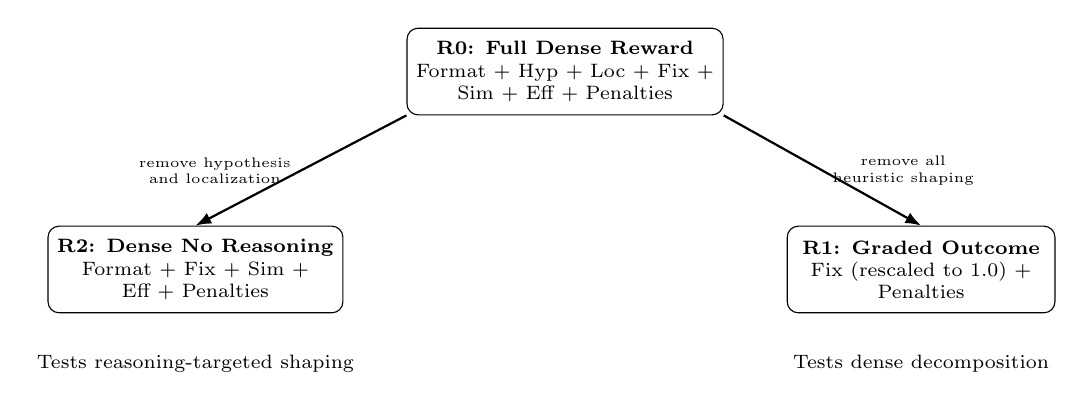
\begin{tikzpicture}[
    rewardbox/.style={
        draw,
        rounded corners,
        align=center,
        minimum width=3.4cm,
        minimum height=1.1cm,
        font=\scriptsize
    },
    arrow/.style={-{Latex[length=2mm]}, thick},
    label/.style={font=\tiny, align=center}
]

\node[rewardbox] (r0) {\textbf{R0: Full Dense Reward}\\Format + Hyp + Loc + Fix +\\Sim + Eff + Penalties};

\node[rewardbox, below left=1.4cm and 0.8cm of r0] (r2)
    {\textbf{R2: Dense No Reasoning}\\Format + Fix + Sim +\\Eff + Penalties};

\node[rewardbox, below right=1.4cm and 0.8cm of r0] (r1)
    {\textbf{R1: Graded Outcome}\\Fix (rescaled to 1.0) +\\Penalties};

\draw[arrow]
    (r0.south west) -- node[label, left]
    {remove hypothesis\\and localization}
    (r2.north);

\draw[arrow]
    (r0.south east) -- node[label, right]
    {remove all\\heuristic shaping}
    (r1.north);

\node[font=\scriptsize, below=0.4cm of r2]
    {Tests reasoning-targeted shaping};

\node[font=\scriptsize, below=0.4cm of r1]
    {Tests dense decomposition};

\end{tikzpicture}
\caption{Three reward configurations used in the controlled experiment, with component decompositions shown. R0--R1 tests whether dense reward decomposition improves performance; R0--R2 tests whether reasoning-targeted components contribute additional benefit; R2--R1 tests whether the remaining non-reasoning shaping terms contribute benefit.}
\label{fig:reward_flow}
\end{figure}

\begin{table}[h]
\centering
\small
\begin{tabular}{l c c c c l}
\toprule
\textbf{Component} & \textbf{R0} & \textbf{R1} & \textbf{R2} & \textbf{Maximum} & \textbf{Purpose} \\
\midrule
Format & \checkmark & --- & \checkmark & 0.10 & Five required response fields \\
Hypothesis & \checkmark & --- & --- & 0.20 & Grounded diagnosis \\
Localization & \checkmark & --- & --- & 0.15 & Function/line ID \\
Fix quality & \checkmark & \checkmark & \checkmark & 0.35 / 1.0 & Tests passed \\
Similarity & \checkmark & --- & \checkmark & 0.10 & Reference proximity \\
Efficiency & \checkmark & --- & \checkmark & 0.10 & Remaining-turn potential \\
Penalties & \checkmark & \checkmark & \checkmark & $-0.55$ & Invalid/regression \\
\bottomrule
\end{tabular}
\caption{Reward components across configurations. In R1, the Fix Quality ceiling is rescaled to 1.0 so that the total reward range is preserved.}
\label{tab:reward_components}
\end{table}

\subsection{Training}
We train Qwen2.5-Coder-3B-Instruct using GRPO with LoRA on the 90 training bugs for 500 optimizer steps. For the 24\,GB GPU profile used in the reported runs, LoRA uses rank 8 and $\alpha=16$, with batch size 2, gradient accumulation of 4, and group size $G=2$. We use AdamW with learning rate $2\times10^{-5}$, cosine scheduling, 30 warmup steps in the first curriculum stage, and sampling temperature 0.7. The curriculum exposes tier 1 for steps 0--149, tiers 1--2 for steps 150--349, and all three tiers for steps 350--499. All three RL configurations use the same training configuration and differ only in reward definition. Full hyperparameters are provided in Appendix~\ref{app:hyperparams}.

\section{Experimental Design}

\subsection{Research Questions}
\begin{itemize}
\item \textbf{RQ1:} Does GRPO training improve held-out debugging?
\item \textbf{RQ2:} Does dense decomposition help? (R0 vs R1)
\item \textbf{RQ3:} Do reasoning-targeted components help? (R0 vs R2)
\item \textbf{RQ4:} Do trained policies transfer beyond the mutation-generated training distribution?
\end{itemize}

\subsection{Experimental Arms}
We conduct 3 independent training runs (seeds 42, 123, 456) for each of the three reward configurations (R0, R1, R2), producing 9 trained policies. We also evaluate the zero-shot base model (B0).

\subsection{Evaluation}
Final evaluations use greedy decoding (temperature 0.0) on the 90 held-out bugs. We also conduct an exploratory external evaluation on 27 single-function adapted QuixBugs programs.

\subsection{Statistical Analysis}
Our primary analysis uses bug-level paired bootstrap intervals, averaging solve indicators across the three seeds before resampling bugs. For each bug $i$, we compute the seed-averaged solve indicator $\bar{s}_{i,\text{arm}} = \frac{1}{3}\sum_{k=1}^{3}s_{i,\text{arm},k}$. We bootstrap the $N=90$ bugs to compute the difference $\Delta = \frac{1}{N}\sum_i (\bar{s}_{i,\text{arm}_A}-\bar{s}_{i,\text{arm}_B})$. The primary bootstrap resamples evaluation bugs and therefore quantifies uncertainty over the evaluation-bug population conditional on the three observed training seeds; it does not provide a reliable estimate of seed-to-seed variance. With 90 paired bugs, the study is powered primarily for relatively large paired effects; effects of only a few percentage points could remain undetected. As a secondary sensitivity analysis, we apply exact McNemar tests to binary paired outcomes defined at the bug level by majority vote across seeds (a bug is solved if $\ge 2/3$ seeds solve it), as well as per-seed paired evaluations (Appendix~\ref{app:stats}); across all comparisons, no contrast approaches significance after Holm--Bonferroni correction.

\paragraph{Deviations from Preregistration.}
The final study differs from the preregistered design in three material ways: model scale (3B instead of 7B), omitted hypotheses (H1 and H3 were dropped), and a calibration baseline change (Llama-3.1-8B-Instruct gating instead of GPT-4o-mini). These changes were made before the final analysis because of compute constraints. No results from the omitted hypotheses are presented as confirmatory evidence.

\begin{table*}[t]
\centering
\small
\begin{tabular}{l c c l}
\toprule
\textbf{Comparison} & \textbf{Contrast} & \textbf{Prediction} & \textbf{Outcome} \\
\midrule
RQ2 & R0 vs R1 & Dense decomposition helps & Not supported \\
RQ3 & R0 vs R2 & Reasoning terms help & Not supported \\
Exploratory & R2 vs R1 & Non-reasoning shaping helps & Not supported \\
Transfer & External evaluation & Nontrivial transfer & Observed \\
\bottomrule
\end{tabular}
\caption{Summary of research questions, contrasts, predictions, and empirical outcomes.}
\label{tab:hypotheses}
\end{table*}

\section{Results}

\begin{table}[h]
\centering
\small
\begin{tabular}{l c c c}
\toprule
\textbf{Model} & \textbf{Train (In-Dist.)} & \textbf{Held-out (In-Dist.)} & \textbf{QuixBugs (External)} \\
\midrule
B0 (Base Zero-Shot) & 37.8\% & 37.8\% & --- \\
E1 (R0 Full)        & 51.9\% $\pm$ 2.3 & 45.6\% $\pm$ 2.9 & 39.5\% $\pm$ 2.1 \\
E3 (R1 Graded Outcome) & 54.4\% $\pm$ 3.3 & 48.5\% $\pm$ 6.5 & 43.2\% $\pm$ 5.7 \\
E4 (R2 No Reasoning)& 51.5\% $\pm$ 3.6 & 48.5\% $\pm$ 3.9 & 44.4\% $\pm$ 3.7 \\
\bottomrule
\end{tabular}
\caption{Solve rate by split and RL configuration (Mean \% $\pm$ Std Dev across 3 seeds). QuixBugs values are descriptive; no zero-shot B0 baseline was evaluated on this external benchmark, so they do not quantify an RL transfer effect.}
\label{tab:results}
\end{table}

\subsection{Main Reward Comparison (Confirmatory)}
\textbf{Main result.} The full dense reward does not improve held-out debugging success relative to either ablated configuration. R0 solves 45.6\% of held-out bugs, versus 48.5\% for both R1 and R2. The point estimate therefore favors the simpler configurations, but the paired bootstrap interval for R0$-$R1, [$-$8.5, $+$2.6] percentage points, includes zero. We interpret this as a null result with respect to detectable improvement, not evidence that the configurations are exactly equivalent.

\begin{table}[h]
\centering
\small
\begin{tabular}{l c c c}
\toprule
\textbf{Comparison} & \textbf{$\Delta$ Solve Rate} & \textbf{95\% Bootstrap CI} & \textbf{Holm-adjusted McNemar $p$} \\
\midrule
R0 $-$ R1 & $-$2.9 pp & [$-$8.5, $+$2.6] & 1.0000 \\
R0 $-$ R2 & $-$2.9 pp & [$-$7.4, $+$1.9] & 1.0000 \\
R2 $-$ R1 & 0.0 pp & [$-$5.9, $+$5.6] & 1.0000 \\
\bottomrule
\end{tabular}
\caption{Pairwise comparisons for held-out solve rates. All bootstrap intervals cross zero, and paired McNemar tests yield no statistically significant difference after Holm correction.}
\label{tab:pairwise}
\end{table}

All three pairwise comparisons yield no statistically detectable difference after Holm correction. Reasoning-targeted reward engineering, at this scale and task, bought no measurable performance.

\subsection{Reward Degeneracy (Exploratory)}
The reward configurations produce substantially different GRPO training signals. Across logged training calls, the mean fraction of degenerate sampled groups (where all samples in a group receive rewards within the configured degeneracy tolerance $\Delta R < 10^{-6}$, resulting in zero relative advantage) was 16.2\% $\pm$ 2.2\% for R0 (individual seed means: 14.4\%, 15.6\%, 18.6\%), 61.9\% $\pm$ 4.2\% for R1 (seed means: 62.3\%, 65.9\%, 57.5\%), and 34.7\% $\pm$ 3.9\% for R2 (seed means: 38.3\%, 30.5\%, 35.3\%). The dense reward substantially reduces the frequency of groups in which sampled completions receive indistinguishable outcomes ($R0 - R1 = -45.7$ pp).

\begin{figure*}[t]
\centering
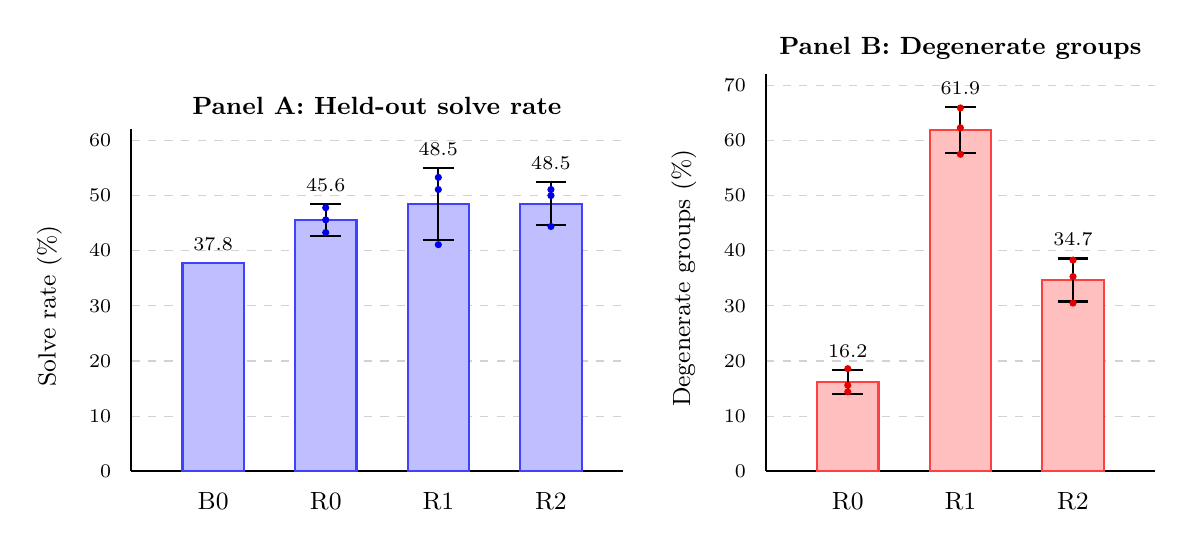
\begin{tikzpicture}[x=1.3cm, y=0.07cm]
    % Left Panel: Solve rate
    \begin{scope}[shift={(0,0)}]
        \foreach \y in {0, 10, 20, 30, 40, 50, 60} {
            \draw[dashed, gray!35] (0, \y) -- (4.8, \y);
            \node[anchor=east, font=\scriptsize] at (-0.1, \y) {\y};
        }
        \draw[thick] (0,0) -- (4.8,0);
        \draw[thick] (0,0) -- (0,62);
        \node[rotate=90, font=\small, anchor=center] at (-0.8, 30) {Solve rate (\%)};
        
        % B0
        \draw[fill=blue!25, draw=blue!75, thick] (0.5,0) rectangle (1.1, 37.8);
        \node[font=\scriptsize, anchor=south] at (0.8, 38.3) {37.8};
        \node[font=\small, anchor=north] at (0.8, -2) {B0};
        
        % R0
        \draw[fill=blue!25, draw=blue!75, thick] (1.6,0) rectangle (2.2, 45.6);
        \draw[thick] (1.9, 45.6 - 2.9) -- (1.9, 45.6 + 2.9);
        \draw[thick] (1.75, 45.6 - 2.9) -- (2.05, 45.6 - 2.9);
        \draw[thick] (1.75, 45.6 + 2.9) -- (2.05, 45.6 + 2.9);
        \fill[blue!90!black] (1.9, 43.3) circle (1.3pt);
        \fill[blue!90!black] (1.9, 45.6) circle (1.3pt);
        \fill[blue!90!black] (1.9, 47.8) circle (1.3pt);
        \node[font=\scriptsize, anchor=south] at (1.9, 49.0) {45.6};
        \node[font=\small, anchor=north] at (1.9, -2) {R0};
        
        % R1
        \draw[fill=blue!25, draw=blue!75, thick] (2.7,0) rectangle (3.3, 48.5);
        \draw[thick] (3.0, 48.5 - 6.5) -- (3.0, 48.5 + 6.5);
        \draw[thick] (2.85, 48.5 - 6.5) -- (3.15, 48.5 - 6.5);
        \draw[thick] (2.85, 48.5 + 6.5) -- (3.15, 48.5 + 6.5);
        \fill[blue!90!black] (3.0, 41.1) circle (1.3pt);
        \fill[blue!90!black] (3.0, 51.1) circle (1.3pt);
        \fill[blue!90!black] (3.0, 53.3) circle (1.3pt);
        \node[font=\scriptsize, anchor=south] at (3.0, 55.5) {48.5};
        \node[font=\small, anchor=north] at (3.0, -2) {R1};
        
        % R2
        \draw[fill=blue!25, draw=blue!75, thick] (3.8,0) rectangle (4.4, 48.5);
        \draw[thick] (4.1, 48.5 - 3.9) -- (4.1, 48.5 + 3.9);
        \draw[thick] (3.95, 48.5 - 3.9) -- (4.25, 48.5 - 3.9);
        \draw[thick] (3.95, 48.5 + 3.9) -- (4.25, 48.5 + 3.9);
        \fill[blue!90!black] (4.1, 44.4) circle (1.3pt);
        \fill[blue!90!black] (4.1, 50.0) circle (1.3pt);
        \fill[blue!90!black] (4.1, 51.1) circle (1.3pt);
        \node[font=\scriptsize, anchor=south] at (4.1, 52.9) {48.5};
        \node[font=\small, anchor=north] at (4.1, -2) {R2};
        
        \node[font=\small\bfseries, anchor=south] at (2.4, 63) {Panel A: Held-out solve rate};
    \end{scope}

    % Right Panel: Degenerate groups
    \begin{scope}[shift={(6.2,0)}]
        \foreach \y in {0, 10, 20, 30, 40, 50, 60, 70} {
            \draw[dashed, gray!35] (0, \y) -- (3.8, \y);
            \node[anchor=east, font=\scriptsize] at (-0.1, \y) {\y};
        }
        \draw[thick] (0,0) -- (3.8,0);
        \draw[thick] (0,0) -- (0,72);
        \node[rotate=90, font=\small, anchor=center] at (-0.8, 35) {Degenerate groups (\%)};
        
        % R0: 16.2 +- 2.2
        \draw[fill=red!25, draw=red!75, thick] (0.5,0) rectangle (1.1, 16.2);
        \draw[thick] (0.8, 16.2 - 2.2) -- (0.8, 16.2 + 2.2);
        \draw[thick] (0.65, 16.2 - 2.2) -- (0.95, 16.2 - 2.2);
        \draw[thick] (0.65, 16.2 + 2.2) -- (0.95, 16.2 + 2.2);
        \fill[red!90!black] (0.8, 14.4) circle (1.3pt);
        \fill[red!90!black] (0.8, 15.6) circle (1.3pt);
        \fill[red!90!black] (0.8, 18.6) circle (1.3pt);
        \node[font=\scriptsize, anchor=south] at (0.8, 18.9) {16.2};
        \node[font=\small, anchor=north] at (0.8, -2) {R0};
        
        % R1: 61.9 +- 4.2
        \draw[fill=red!25, draw=red!75, thick] (1.6,0) rectangle (2.2, 61.9);
        \draw[thick] (1.9, 61.9 - 4.2) -- (1.9, 61.9 + 4.2);
        \draw[thick] (1.75, 61.9 - 4.2) -- (2.05, 61.9 - 4.2);
        \draw[thick] (1.75, 61.9 + 4.2) -- (2.05, 61.9 + 4.2);
        \fill[red!90!black] (1.9, 57.5) circle (1.3pt);
        \fill[red!90!black] (1.9, 62.3) circle (1.3pt);
        \fill[red!90!black] (1.9, 65.9) circle (1.3pt);
        \node[font=\scriptsize, anchor=south] at (1.9, 66.6) {61.9};
        \node[font=\small, anchor=north] at (1.9, -2) {R1};
        
        % R2: 34.7 +- 3.9
        \draw[fill=red!25, draw=red!75, thick] (2.7,0) rectangle (3.3, 34.7);
        \draw[thick] (3.0, 34.7 - 3.9) -- (3.0, 34.7 + 3.9);
        \draw[thick] (2.85, 34.7 - 3.9) -- (3.15, 34.7 - 3.9);
        \draw[thick] (2.85, 34.7 + 3.9) -- (3.15, 34.7 + 3.9);
        \fill[red!90!black] (3.0, 30.5) circle (1.3pt);
        \fill[red!90!black] (3.0, 35.3) circle (1.3pt);
        \fill[red!90!black] (3.0, 38.3) circle (1.3pt);
        \node[font=\scriptsize, anchor=south] at (3.0, 39.1) {34.7};
        \node[font=\small, anchor=north] at (3.0, -2) {R2};
        
        \node[font=\small\bfseries, anchor=south] at (1.9, 73) {Panel B: Degenerate groups};
    \end{scope}
\end{tikzpicture}
\caption{Held-out solve rate and GRPO reward degeneracy. Bars show mean values across three seeds; error bars indicate standard deviation across seeds, with filled dots displaying individual seed runs. Degeneracy values show the mean fraction of degenerate sampled groups across the three seeds, with error bars showing the standard deviation across seed-level means. The dense reward substantially changes the training signal while producing no detectable improvement in held-out solve rate.}
\label{fig:main_results}
\end{figure*}

However, this difference does not translate into higher held-out solve rate. R1 also exhibits greater across-seed variance (std dev $\pm 6.5$ vs $\pm 2.9$), consistent with---but insufficient to establish---the hypothesis that increased reward degeneracy produces noisier, less stable optimization. Three seeds are insufficient for a formal variance comparison. This establishes an association between reward configuration and group degeneracy, not a causal relationship between degeneracy and final performance.

\subsection{Training vs Held-out (Confirmatory)}
Pooling the nine RL runs gives a mean held-out solve rate of 47.5\%, 9.7 percentage points above B0's 37.8\% (bootstrap 95\% CI [1.0, 18.5]). This pooled comparison is descriptive and should not be interpreted as a single-model estimate of the effect of RL. The effect is not individually significant for E1 under the same bootstrap analysis. The train--held-out gap is approximately 6 percentage points. This gap is descriptively modest, although the experiment is not designed to distinguish generalization from other sources of train--held-out differences.

\subsection{External-Source Transfer (Exploratory)}
We evaluate the trained policies on a 27-program external set adapted from QuixBugs. E1, E3, and E4 achieve 39.5\% $\pm$ 2.1\%, 43.2\% $\pm$ 5.7\%, and 44.4\% $\pm$ 3.7\%, respectively. These numbers establish that the policies maintain basic repair capability outside the synthetic MBPP mutation distribution. However, because we did not evaluate an untrained zero-shot B0 baseline on this external set, these measurements cannot distinguish whether this performance reflects transfer acquired through RL training or simply the base model's pre-existing code generation competence. We therefore report them strictly as descriptive out-of-distribution observations rather than evidence of an RL transfer advantage.

\subsection{Evaluation-Harness Failure Analysis (Exploratory)}
Our initial zero-shot experiments produced a surprising artifact. An artificial truncation error vastly suppressed free-form code generation success.

\begin{table}[h]
\centering
\small
\begin{tabular}{l c c c}
\toprule
\textbf{Configuration} & \textbf{Max tokens} & \textbf{Extraction failure} & \textbf{Solve rate} \\
\midrule
B1 initial & 300 & 86.7\% & 1.1\% \\
B1 corrected & 700 & < 5.0\% & 45.6\% \\
B0 structured & 700 & < 5.0\% & 37.8\% \\
\bottomrule
\end{tabular}
\caption{Impact of generation budget on evaluation fidelity.}
\label{tab:truncation}
\end{table}

Increasing the budget to 700 tokens largely eliminated the truncation-induced discrepancy. A separate evaluation-harness error reduced the observed free-form solve rate from 45.6\% to 1.1\%, creating a 44.5-point apparent performance difference that dwarfed the reward effects studied here. The evaluation-harness incident illustrates why artifact validation is part of experimental methodology rather than a peripheral engineering concern.

\section{Discussion}
The seven-component reward introduces hundreds of lines of heuristic scoring logic and several independently chosen design thresholds, each introducing an additional opportunity for reward misspecification or exploitation. Despite this engineering effort, the simpler graded outcome reward was sufficient to achieve comparable held-out performance. 

\subsection{Why Did Dense Reward Fail to Improve Solve Rate?}
One possibility is that executable test outcomes already provide sufficiently informative gradients for this base model. A second is that the additional heuristic components are only weakly correlated with successful repairs. A third is that single-turn generation removes the temporal credit-assignment problem for which intermediate rewards are most naturally useful. This setting may therefore be unusually unfavorable to process-oriented reward shaping: the model emits a complete fix in one completion, so there is no temporal sequence over which intermediate diagnostic rewards can improve credit assignment. Finally, with group size $G=2$, reducing reward degeneracy may alter gradient availability without increasing the quality of the underlying optimization direction. 

Importantly, these explanations are not distinguished by the present experiment: the data establish that reward configuration changes group-level reward degeneracy, but not why that change fails to improve final repair accuracy.

\section{Limitations and Scope}
\begin{itemize}
\item \textbf{Model scale:} Only Qwen2.5-Coder-3B.
\item \textbf{Algorithm:} Only GRPO.
\item \textbf{Group size:} Only $G=2$. With $G=2$, a single sampled success creates maximal contrast, and identical rewards create zero variance. Larger groups might reduce the importance of reward decomposition.
\item \textbf{Task structure:} Single-function, single-turn. Multi-step debugging may present a different regime in which intermediate rewards could be substantially more valuable.
\item \textbf{Bug distribution:} Mutation-generated MBPP bugs.
\item \textbf{Transfer set:} Only 27 adapted QuixBugs programs evaluated without a zero-shot baseline, rendering external numbers descriptive.
\item \textbf{Seeds:} Only 3 per arm, limiting robust variance estimates.
\item \textbf{Statistical power:} Large paired effects are detectable; small effects of a few percentage points are not.
\item \textbf{Reward design:} Our ``dense reward'' is one particular handcrafted design, not all dense rewards. This study does not establish that dense rewards do not work, only that this specific decomposition did not improve this task.
\end{itemize}

\paragraph{What this study does NOT establish.}
Dense reward shaping never helps; Outcome reward is universally sufficient; Reasoning rewards are useless; GRPO is superior to other RL algorithms; 3B debugging results transfer to frontier models; Single-turn debugging results apply to agentic repository-level debugging; QuixBugs establishes robust generalization.

\section{Conclusion}
The most informative result is not simply that the dense reward failed to improve solve rate. It is that it changed the optimization signal substantially: R0 produced far fewer degenerate GRPO groups than R1, yet this advantage did not translate into higher held-out performance. This suggests that, in a regime where the base model already obtains meaningful executable feedback and the action is a complete single-turn fix, additional heuristic reward signal may improve reward resolution without improving the learned policy. The result therefore separates two quantities that are often implicitly conflated: reward resolution within a GRPO group and the usefulness of the resulting optimization direction. Furthermore, a separate evaluation-harness error reduced the observed free-form solve rate from 45.6\% to 1.1\%, creating a 44.5-point apparent performance difference that dwarfed the reward effects studied here.

\textbf{Practical takeaway.} If a code-RL system already obtains meaningful executable feedback from a moderately capable base model, first establish that the outcome reward is insufficient before introducing additional heuristic reasoning rewards. Such shaping may reduce reward degeneracy, but our results show that this optimization benefit need not translate into better final repair accuracy.

\bibliographystyle{plain}
\begin{thebibliography}{9}
\bibitem{Austin2021} Austin, J., Odena, A., Nye, M., et al. (2021). Program Synthesis with Large Language Models. arXiv:2108.07732.
\bibitem{Guo2025} Guo, D., et al. (2025). DeepSeek-R1: Incentivizing Reasoning Capability in LLMs via Reinforcement Learning. arXiv:2501.12948.
\bibitem{Lightman2023} Lightman, H., et al. (2023). Let's Verify Step by Step. ICLR 2024. arXiv:2305.20050.
\bibitem{Lin2017} Lin, D., et al. (2017). QuixBugs: A Multi-Lingual Program Repair Benchmark Set Based on the Quixey Challenge. SPLASH Companion 2017.
\bibitem{McNemar1947} McNemar, Q. (1947). Note on the sampling error of the difference between correlated proportions or percentages. Psychometrika, 12(2), 153--157.
\bibitem{Ng1999} Ng, A. Y., Harada, D., \& Russell, S. (1999). Policy invariance under reward transformations: Theory and application to reward shaping. ICML 1999.
\bibitem{Shao2024} Shao, Z., et al. (2024). DeepSeekMath: Pushing the Limits of Mathematical Reasoning in Open Language Models. arXiv:2402.03300.
\bibitem{Tam2024} Tam, Z. R., et al. (2024). Let Me Speak Freely? Long-Form Thinking and Evaluation Artifacts. EMNLP 2024. arXiv:2408.02442.
\bibitem{Tian2024} Tian, R., et al. (2024). DebugBench: Evaluating Large Language Models for Program Debugging. ACL 2024. arXiv:2401.04621.
\bibitem{Uesato2022} Uesato, J., et al. (2022). Solving Math Word Problems with Process- and Outcome-based Feedback. arXiv:2211.14275.
\end{thebibliography}

\clearpage
\appendix

\section{Training Hyperparameters}
\label{app:hyperparams}

Table~\ref{tab:hyperparams} reports the training hyperparameters for the reported 24\,GB GPU runs. All reward component ceilings and penalty magnitudes were fixed in the pre-registered environment specification before the reported training runs; they were not tuned against held-out solve rates. The curriculum schedule is given in Table~\ref{tab:curriculum}.

\begin{table}[h]
\centering
\small
\begin{tabular}{ll}
\toprule
\textbf{Parameter} & \textbf{Value} \\
\midrule
Base model & Qwen/Qwen2.5-Coder-3B-Instruct \\
RL algorithm & GRPO \\
LoRA rank & 8 \\
LoRA $\alpha$ & 16 \\
LoRA dropout & 0.0 \\
LoRA target modules & q\_proj, k\_proj, v\_proj, o\_proj, gate\_proj, up\_proj, down\_proj \\
Optimizer & AdamW \\
Learning rate & $2\times10^{-5}$ \\
Scheduler & cosine \\
Warmup & 30 steps (stage 1 only) \\
Total optimizer steps & 500 \\
Group size $G$ & 2 \\
Per-device batch size & 2 \\
Gradient accumulation steps & 4 \\
Generations per prompt & 2 \\
Structured completion budget & 192 tokens \\
Sampling temperature & 0.7 \\
Reward workers & 1 \\
Seeds & 42, 123, 456 \\
\bottomrule
\end{tabular}
\caption{Training hyperparameters for the reported 24\,GB GPU runs.}
\label{tab:hyperparams}
\end{table}

\begin{table}[h]
\centering
\small
\begin{tabular}{c c l}
\toprule
\textbf{Curriculum Stage} & \textbf{Training Steps} & \textbf{Active Tiers} \\
\midrule
Stage 0 & 0--149 & Tier 1 (Easy) \\
Stage 1 & 150--349 & Tiers 1--2 (Easy, Medium) \\
Stage 2 & 350--499 & Tiers 1--3 (Easy, Medium, Hard) \\
\bottomrule
\end{tabular}
\caption{Curriculum schedule used in all three RL configurations.}
\label{tab:curriculum}
\end{table}

\paragraph{Curriculum-stage optimization.}
Training is implemented as three sequential GRPO trainers, one per curriculum stage. The LoRA adapter is carried across stages, while each stage initializes a fresh optimizer and scheduler. Only the first stage uses the 30-step warmup; later stages restart the cosine schedule at the configured learning rate without warmup. This implementation detail is shared across R0, R1, and R2.

\section{Statistical Analysis Details}
\label{app:stats}

\subsection{Primary Paired Bootstrap}
For each bug $i \in \{1, \dots, 90\}$, the solve indicator is averaged across the three seeds:
\begin{equation}
\bar{s}_{i,\text{arm}} = \frac{1}{3}\sum_{k=1}^{3} s_{i,\text{arm},k}
\end{equation}
The analysis script also verifies that all nine RL result files contain the same 90 held-out bug identifiers and that the train and held-out bug IDs are disjoint before computing intervals. We resample the $N=90$ bugs with replacement 10,000 times (fixed RNG seed 204) to generate the empirical distribution of paired differences $\Delta = \frac{1}{N}\sum_{i=1}^{N}(\bar{s}_{i,\text{arm}_A} - \bar{s}_{i,\text{arm}_B})$. Percentile endpoints at 2.5\% and 97.5\% define the 95\% confidence intervals.

\subsection{Secondary McNemar Sensitivity Analysis}
To evaluate sensitivity, we apply exact paired binomial McNemar tests to discordant pairs. For the majority-vote analysis, all three Holm-adjusted $p$-values are 1.0000. The per-seed sensitivity analyses likewise yield no statistically significant contrast after Holm correction; the smallest adjusted $p$-value is 0.2780.

\begin{table}[h]
\centering
\small
\begin{tabular}{l c c c c c c}
\toprule
\textbf{Comparison} & \textbf{Arm A Solved} & \textbf{Arm B Solved} & \textbf{A-only} & \textbf{B-only} & \textbf{Raw $p$} & \textbf{Holm-adj $p$} \\
\midrule
E1 vs E3 & 42/90 (46.7\%) & 44/90 (48.9\%) & 8 & 10 & 0.8145 & 1.0000 \\
E1 vs E4 & 42/90 (46.7\%) & 44/90 (48.9\%) & 6 & 8 & 0.7905 & 1.0000 \\
E3 vs E4 & 44/90 (48.9\%) & 44/90 (48.9\%) & 7 & 7 & 1.0000 & 1.0000 \\
\bottomrule
\end{tabular}
\caption{Majority-vote McNemar tests on held-out bugs (a bug is considered solved if solved by $\ge 2/3$ seeds).}
\label{tab:mcnemar_majority}
\end{table}

\begin{table}[h]
\centering
\small
\begin{tabular}{l c c c c c c}
\toprule
\textbf{Comparison} & \textbf{Seed} & \textbf{A-only} & \textbf{B-only} & \textbf{Discordant} & \textbf{Raw $p$} & \textbf{Holm-adj $p$} \\
\midrule
E1 vs E3 & s42  & 13 & 7  & 20 & 0.2632 & 1.0000 \\
E1 vs E3 & s123 & 12 & 16 & 28 & 0.5716 & 1.0000 \\
E1 vs E3 & s456 & 5  & 15 & 20 & 0.0414 & 0.3311 \\
E1 vs E4 & s42  & 9  & 13 & 22 & 0.5235 & 1.0000 \\
E1 vs E4 & s123 & 7  & 9  & 16 & 0.8036 & 1.0000 \\
E1 vs E4 & s456 & 9  & 11 & 20 & 0.8238 & 1.0000 \\
E3 vs E4 & s42  & 4  & 14 & 18 & 0.0309 & 0.2780 \\
E3 vs E4 & s123 & 12 & 10 & 22 & 0.8318 & 1.0000 \\
E3 vs E4 & s456 & 12 & 4  & 16 & 0.0768 & 0.5377 \\
\bottomrule
\end{tabular}
\caption{Per-seed exact McNemar tests across the 9 individual runs.}
\label{tab:mcnemar_perseed}
\end{table}

\section{External Transfer Set (QuixBugs)}
\label{app:quixbugs}

The external transfer benchmark consists of 27 single-function Python programs adapted from the QuixBugs dataset \cite{Lin2017}. Out of 40 original QuixBugs programs, 13 were excluded because their argument or return shapes required custom pointer/graph structures not representable in JSON (e.g., linked list or graph nodes) or used generator yields without list wrapping. 

The 27 validated candidate programs are listed in Table~\ref{tab:quixbugs_list}. All programs were verified with our sandbox validator: the reference code passes 100\% of test cases, and the buggy code fails at least one case. Because no zero-shot B0 baseline was executed on this external set, performance is reported descriptively.

\begin{table}[h]
\centering
\footnotesize
\begin{tabular}{lll}
\toprule
\multicolumn{3}{c}{\textbf{QuixBugs Program Identifiers (27 Programs)}} \\
\midrule
\texttt{quixbugs\_bitcount} & \texttt{quixbugs\_bucketsort} & \texttt{quixbugs\_find\_first\_in\_sorted} \\
\texttt{quixbugs\_find\_in\_sorted} & \texttt{quixbugs\_gcd} & \texttt{quixbugs\_get\_factors} \\
\texttt{quixbugs\_is\_valid\_parenthesization} & \texttt{quixbugs\_knapsack} & \texttt{quixbugs\_kth} \\
\texttt{quixbugs\_lcs\_length} & \texttt{quixbugs\_levenshtein} & \texttt{quixbugs\_lis} \\
\texttt{quixbugs\_longest\_common\_subsequence} & \texttt{quixbugs\_max\_sublist\_sum} & \texttt{quixbugs\_mergesort} \\
\texttt{quixbugs\_next\_palindrome} & \texttt{quixbugs\_next\_permutation} & \texttt{quixbugs\_pascal} \\
\texttt{quixbugs\_possible\_change} & \texttt{quixbugs\_powerset} & \texttt{quixbugs\_quicksort} \\
\texttt{quixbugs\_rpn\_eval} & \texttt{quixbugs\_shunting\_yard} & \texttt{quixbugs\_sieve} \\
\texttt{quixbugs\_subsequences} & \texttt{quixbugs\_to\_base} & \texttt{quixbugs\_wrap} \\
\bottomrule
\end{tabular}
\caption{Identifiers of the 27 adapted QuixBugs programs used for external transfer evaluation.}
\label{tab:quixbugs_list}
\end{table}

\section{Artifact Reproducibility}
\label{app:artifact}

Table~\ref{tab:artifacts} lists the primary repository locations of all datasets, rewards, training pipelines, and results.

\begin{table}[h]
\centering
\small
\begin{tabular}{ll}
\toprule
\textbf{Artifact} & \textbf{Location} \\
\midrule
Dataset & \texttt{data/v2/} \\
Fixed train/held-out split & \texttt{src/agentdebugger/dataset/bugs/} \\
QuixBugs external set & \texttt{data/quixbugs/} \\
Reward implementation & \texttt{src/agentdebugger/rewards/} \\
Curriculum environment & \texttt{src/agentdebugger/envs/curriculum\_env.py} \\
Training implementation & \texttt{src/agentdebugger/training/grpo.py} \\
Per-run evaluation results & \texttt{results/primary/E*\_s*.json} \\
Diagnostic evaluations & \texttt{results/diagnostics/} \\
Statistical analysis scripts & \texttt{analysis/bootstrap.py}, \texttt{analysis/analyze\_wandb.py} \\
Dataset construction & \texttt{scripts/build\_dataset.py} \\
QuixBugs adaptation script & \texttt{scripts/build\_quixbugs.py} \\
\bottomrule
\end{tabular}
\caption{Locations of the primary experimental artifacts in the released repository.}
\label{tab:artifacts}
\end{table}

\section{Evaluation-Harness Failure Analysis}
\label{app:harness}

During preliminary zero-shot evaluation, free-form completions were evaluated with a generation limit of 300 tokens. Free-form responses typically emitted thorough analytical prose before outputting the code fix block. Consequently, completions routinely exhausted the 300-token limit before reaching the closing code fence, resulting in an 86.7\% extraction failure rate and an apparent solve rate of only 1.1\%. 

Increasing the token limit to 700 tokens allowed models to complete both their analytical reasoning and the final code block, dropping extraction failures below 5\% and restoring the solve rate to 45.6\% (a 44.5 percentage point increase). This finding emphasizes that benchmark evaluation harnesses can introduce massive confounding effects that completely overshadow the algorithmic interventions under study.

\clearpage
\section{NeurIPS Paper Checklist}
\label{app:checklist}

\begin{enumerate}

\item[] \textbf{1. Claims} \hfill \textbf{[Yes]}
\item[] \textit{Question:} Do the main claims made in the abstract and introduction accurately reflect the paper's contributions and scope?
\item[] \textit{Answer:} \textbf{Yes.}
\item[] \textit{Justification:} The main claims in the abstract and introduction explicitly match the empirical findings, state the negative results, and provide paired bootstrap confidence intervals. See Sections 1 and 5.

\item[] \textbf{2. Limitations} \hfill \textbf{[Yes]}
\item[] \textit{Question:} Have the authors discussed the limitations of their work?
\item[] \textit{Answer:} \textbf{Yes.}
\item[] \textit{Justification:} Section 7 is dedicated to limitations and scope, detailing model scale (3B), group size ($G=2$), single-turn structure, benchmark distribution, and seed counts.

\item[] \textbf{3. Theory, Assumptions and Proofs} \hfill \textbf{[NA]}
\item[] \textit{Question:} If you are including theoretical results, did you state the full set of assumptions and include complete proofs?
\item[] \textit{Answer:} \textbf{NA.}
\item[] \textit{Justification:} This is an empirical study evaluating reinforcement learning reward decomposition; no formal mathematical proofs or theorems are claimed.

\item[] \textbf{4. Experimental Result Reproducibility} \hfill \textbf{[Yes]}
\item[] \textit{Question:} If the contribution is a dataset or model, what steps did you take to make your results reproducible or verifiable?
\item[] \textit{Answer:} \textbf{Yes.}
\item[] \textit{Justification:} Complete environment specifications, hyperparameters, random seeds, and reproduction steps are provided in Section 4 and Appendices~\ref{app:hyperparams} and~\ref{app:artifact}.

\item[] \textbf{5. Open Access to Data and Code} \hfill \textbf{[Yes]}
\item[] \textit{Question:} Did you include the code, data, and instructions needed to reproduce the main experimental results?
\item[] \textit{Answer:} \textbf{Yes.}
\item[] \textit{Justification:} All code, dataset splits, reward implementations, and evaluation scripts are released in the accompanying artifact repository (Appendix~\ref{app:artifact}).

\item[] \textbf{6. Experimental Setting / Details} \hfill \textbf{[Yes]}
\item[] \textit{Question:} Did you specify all the training details (e.g., data splits, hyperparameters, how they were chosen)?
\item[] \textit{Answer:} \textbf{Yes.}
\item[] \textit{Justification:} Hardware profiles, LoRA ranks, optimizer settings, batch geometry, and curriculum stages are detailed in Section 3.5 and Appendix~\ref{app:hyperparams}.

\item[] \textbf{7. Experiment Statistical Significance} \hfill \textbf{[Yes]}
\item[] \textit{Question:} Does the paper report error bars suitably and correctly defined or other appropriate information about the statistical significance of the experiments?
\item[] \textit{Answer:} \textbf{Yes.}
\item[] \textit{Justification:} We report bug-level paired bootstrap 95\% confidence intervals (10,000 resamples), exact McNemar tests with Holm--Bonferroni correction, and across-seed standard deviations in Section 5 and Appendix~\ref{app:stats}.

\item[] \textbf{8. Experiments Compute Resource} \hfill \textbf{[Yes]}
\item[] \textit{Question:} For each experiment, does the paper provide sufficient information on the computer resources needed to reproduce the experiments?
\item[] \textit{Answer:} \textbf{Yes.}
\item[] \textit{Justification:} Compute resources (24\,GB RTX 4090 GPUs, approx. 75 total GPU hours across calibration, pilots, and the 9 matrix runs) are documented in Section 3.5 and Appendix~\ref{app:hyperparams}.

\item[] \textbf{9. Code of Ethics} \hfill \textbf{[Yes]}
\item[] \textit{Question:} Have you read the NeurIPS Code of Ethics and ensured that your research conforms to it?
\item[] \textit{Answer:} \textbf{Yes.}
\item[] \textit{Justification:} We have read the NeurIPS Code of Ethics and confirmed our research conforms to it.

\item[] \textbf{10. Broader Impacts} \hfill \textbf{[Yes]}
\item[] \textit{Question:} If appropriate for the scope and focus of your paper, did you discuss potential negative societal impacts of your work?
\item[] \textit{Answer:} \textbf{Yes.}
\item[] \textit{Justification:} We study automated code repair in sandboxed environments. While autonomous code modification could theoretically introduce defects if deployed without human oversight, all code execution in this work occurs in an isolated, resource-capped sandbox (Section 3.2).

\item[] \textbf{11. Safeguards} \hfill \textbf{[NA]}
\item[] \textit{Question:} Do you have safeguards in place for responsible release of models with a high risk for misuse?
\item[] \textit{Answer:} \textbf{NA.}
\item[] \textit{Justification:} The released models are small-scale (3B parameter) LoRA adapters fine-tuned solely on single-function Python bug fixes, posing no high risk of misuse or dual-use.

\item[] \textbf{12. Licenses} \hfill \textbf{[Yes]}
\item[] \textit{Question:} If you are using existing assets, did you cite the creators and respect the license and terms of use?
\item[] \textit{Answer:} \textbf{Yes.}
\item[] \textit{Justification:} All existing assets used—MBPP (CC BY 4.0) and QuixBugs (MIT)—are cited and used in compliance with their licenses. Our repository is released under the MIT license.

\item[] \textbf{13. Assets} \hfill \textbf{[Yes]}
\item[] \textit{Question:} If you are releasing new assets, did you document them and provide these details alongside the assets?
\item[] \textit{Answer:} \textbf{Yes.}
\item[] \textit{Justification:} Details of the mutated MBPP dataset (180 bugs) and adapted QuixBugs benchmark (27 programs) are documented with structured data cards and schemas in Appendix~\ref{app:quixbugs} and \texttt{data/quixbugs/DATACARD.md}.

\item[] \textbf{14. Crowdsourcing and Research with Human Subjects} \hfill \textbf{[NA]}
\item[] \textit{Question:} If you used crowdsourcing or conducted research with human subjects, did you include full instructions and compensation details?
\item[] \textit{Answer:} \textbf{NA.}
\item[] \textit{Justification:} This research does not involve human subjects or crowdsourcing.

\item[] \textbf{15. IRB Approvals} \hfill \textbf{[NA]}
\item[] \textit{Question:} Did you describe potential participant risks and obtain Institutional Review Board (IRB) approvals?
\item[] \textit{Answer:} \textbf{NA.}
\item[] \textit{Justification:} No human subjects or sensitive personal data were involved in this work.

\item[] \textbf{16. Declaration of LLM usage} \hfill \textbf{[NA]}
\item[] \textit{Question:} Does the paper describe the usage of LLMs if it is an important, original, or non-standard component of the core methods?
\item[] \textit{Answer:} \textbf{NA.}
\item[] \textit{Justification:} Language models are the object of empirical study in our research, rather than a component used to write, edit, or generate the core findings of the paper.

\end{enumerate}

\end{document}
